
% LaTeX Beamer file automatically generated from DocOnce
% https://github.com/doconce/doconce

%-------------------- begin beamer-specific preamble ----------------------

\documentclass{beamer}

\usetheme{red_plain}
\usecolortheme{default}

% turn off the almost invisible, yet disturbing, navigation symbols:
\setbeamertemplate{navigation symbols}{}

% Examples on customization:
%\usecolortheme[named=RawSienna]{structure}
%\usetheme[height=7mm]{Rochester}
%\setbeamerfont{frametitle}{family=\rmfamily,shape=\itshape}
%\setbeamertemplate{items}[ball]
%\setbeamertemplate{blocks}[rounded][shadow=true]
%\useoutertheme{infolines}
%
%\usefonttheme{}
%\useinntertheme{}
%
%\setbeameroption{show notes}
%\setbeameroption{show notes on second screen=right}

% fine for B/W printing:
%\usecolortheme{seahorse}

\usepackage{pgf}
\usepackage{graphicx}
\usepackage{epsfig}
\usepackage{relsize}

\usepackage{fancybox}  % make sure fancybox is loaded before fancyvrb

\usepackage{fancyvrb}
\usepackage{minted} % requires pygments and latex -shell-escape filename
%\usepackage{anslistings}
%\usepackage{listingsutf8}

\usepackage{amsmath,amssymb,bm}
%\usepackage[latin1]{inputenc}
\usepackage[T1]{fontenc}
\usepackage[utf8]{inputenc}
\usepackage{colortbl}
\usepackage[english]{babel}
\usepackage{tikz}
\usepackage{framed}
% Use some nice templates
\beamertemplatetransparentcovereddynamic

% --- begin table of contents based on sections ---
% Delete this, if you do not want the table of contents to pop up at
% the beginning of each section:
% (Only section headings can enter the table of contents in Beamer
% slides generated from DocOnce source, while subsections are used
% for the title in ordinary slides.)
\AtBeginSection[]
{
  \begin{frame}<beamer>[plain]
  \frametitle{}
  %\frametitle{Outline}
  \tableofcontents[currentsection]
  \end{frame}
}
% --- end table of contents based on sections ---

% If you wish to uncover everything in a step-wise fashion, uncomment
% the following command:

%\beamerdefaultoverlayspecification{<+->}

\newcommand{\shortinlinecomment}[3]{\note{\textbf{#1}: #2}}
\newcommand{\longinlinecomment}[3]{\shortinlinecomment{#1}{#2}{#3}}

\definecolor{linkcolor}{rgb}{0,0,0.4}
\hypersetup{
    colorlinks=true,
    linkcolor=linkcolor,
    urlcolor=linkcolor,
    pdfmenubar=true,
    pdftoolbar=true,
    bookmarksdepth=3
    }
\setlength{\parskip}{0pt}  % {1em}

\newenvironment{doconceexercise}{}{}
\newcounter{doconceexercisecounter}
\newenvironment{doconce:movie}{}{}
\newcounter{doconce:movie:counter}

\newcommand{\subex}[1]{\noindent\textbf{#1}}  % for subexercises: a), b), etc

%-------------------- end beamer-specific preamble ----------------------

% Add user's preamble


% insert custom LaTeX commands...
\raggedbottom
\makeindex
%-------------------- end preamble ----------------------
\begin{document}
% matching end for #ifdef PREAMBLE
\newcommand{\exercisesection}[1]{\subsection*{#1}}
\input{newcommands_bfmath}
\input{newcommands_replace}

% ------------------- main content ----------------------
% ----------------- title -------------------------
\title{On Schemes for Exponential Decay}
% ----------------- author(s) -------------------------
\author{Hans Petter Langtangen\inst{1,2}}
\institute{Center for Biomedical Computing, Simula Research Laboratory\inst{1}
\and
Department of Informatics, University of Oslo\inst{2}}
% ----------------- end author(s) -------------------------
\date{Jan 32, 2100
\\ \ \\ 
\centerline{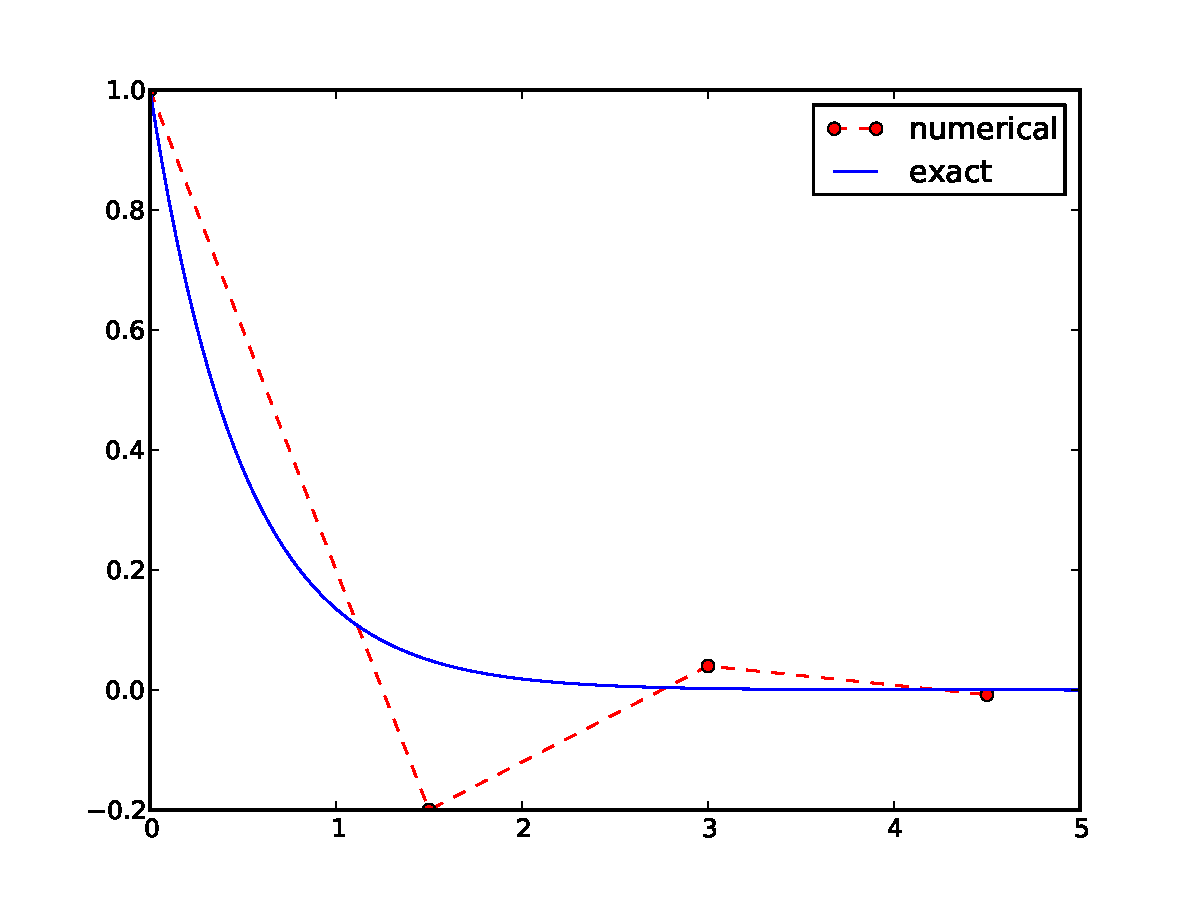
\includegraphics[width=0.4\linewidth]{../doc/src/slides/fig/CN_logo.pdf}}
% <optional copyright>
}
\vspace{6mm}

\vspace{6mm}

\begin{frame}[plain,fragile]
\titlepage
\end{frame}

\begin{frame}[plain,fragile]
\frametitle{Goal}

The primary goal of this demo talk is to demonstrate how to write
talks with \href{{https://github.com/doconce/doconce}}{DocOnce}
and get them rendered in numerous HTML formats.
\begin{block}{Layout }
This version
utilizes beamer slides with the theme red_plain.
\end{block}
\note{
The talk investigates the accuracy of three finite difference
schemes for the ordinary differential equation $u'=-au$ with the
aid of numerical experiments. Numerical artifacts are in particular
demonstrated.
}
\end{frame}

\section{Methods}

\begin{frame}[plain,fragile]
\frametitle{Mathematical problem}

\begin{columns}
\column{0.5\textwidth}
\begin{align}
u'(t) &= -au(t),
\label{ode}\\ 
u(0)  &= I,
\label{initial:value}
\end{align}
\begin{itemize}
 \item $t\in (0,T]$
 \item $a$, $I$, and $T$ are prescribed parameters
 \item $u(t)$ is the unknown function
\end{itemize}
\noindent

\column{0.5\textwidth}
\vspace{6mm}
% inline figure
\centerline{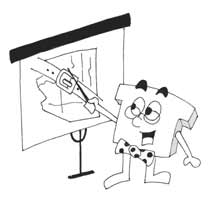
\includegraphics[width=0.5\linewidth]{../doc/src/slides/fig/teacher2.jpg}}
\vspace{6mm}

\end{columns}
\end{frame}

\begin{frame}[plain,fragile]
\frametitle{Numerical solution method}

\begin{itemize}
\pause
 \item Mesh in time: $0= t_0< t_1 \cdots < t_N=T$
\pause
 \item Assume constant $\Delta t = t_{n}-t_{n-1}$
\pause
 \item $u^n$: numerical approx to the exact solution at $t_n$
\end{itemize}
\noindent
\pause
Numerical scheme:
   \[
   u^{n+1} = \frac{1 - (1-\theta) a\Delta t}{1 + \theta a\Delta t}u^n,
   \quad n=0,1,\ldots,N-1
   \]
\end{frame}

\begin{frame}[plain,fragile]
\frametitle{Implementation}

The numerical method is implemented in a Python function:
\begin{minted}[fontsize=\fontsize{9pt}{9pt},linenos=false,mathescape,baselinestretch=1.0,fontfamily=tt,xleftmargin=2mm]{python}
def solver(I, a, T, dt, theta):
    """Solve u'=-a*u, u(0)=I, for t in (0,T]; step: dt."""
    dt = float(dt)           # avoid integer division
    N = int(round(old_div(T,dt)))     # no of time intervals
    T = N*dt                 # adjust T to fit time step dt
    u = zeros(N+1)           # array of u[n] values
    t = linspace(0, T, N+1)  # time mesh

    u[0] = I                 # assign initial condition
    for n in range(0, N):    # n=0,1,...,N-1
        u[n+1] = (1 - (1-theta)*a*dt)/(1 + theta*dt*a)*u[n]
    return u, t

\end{minted}
\end{frame}

\section[Results]{Selected results}

\begin{frame}[plain,fragile]
\frametitle{The Crank-Nicolson method}

\vspace{6mm}
% inline figure
\centerline{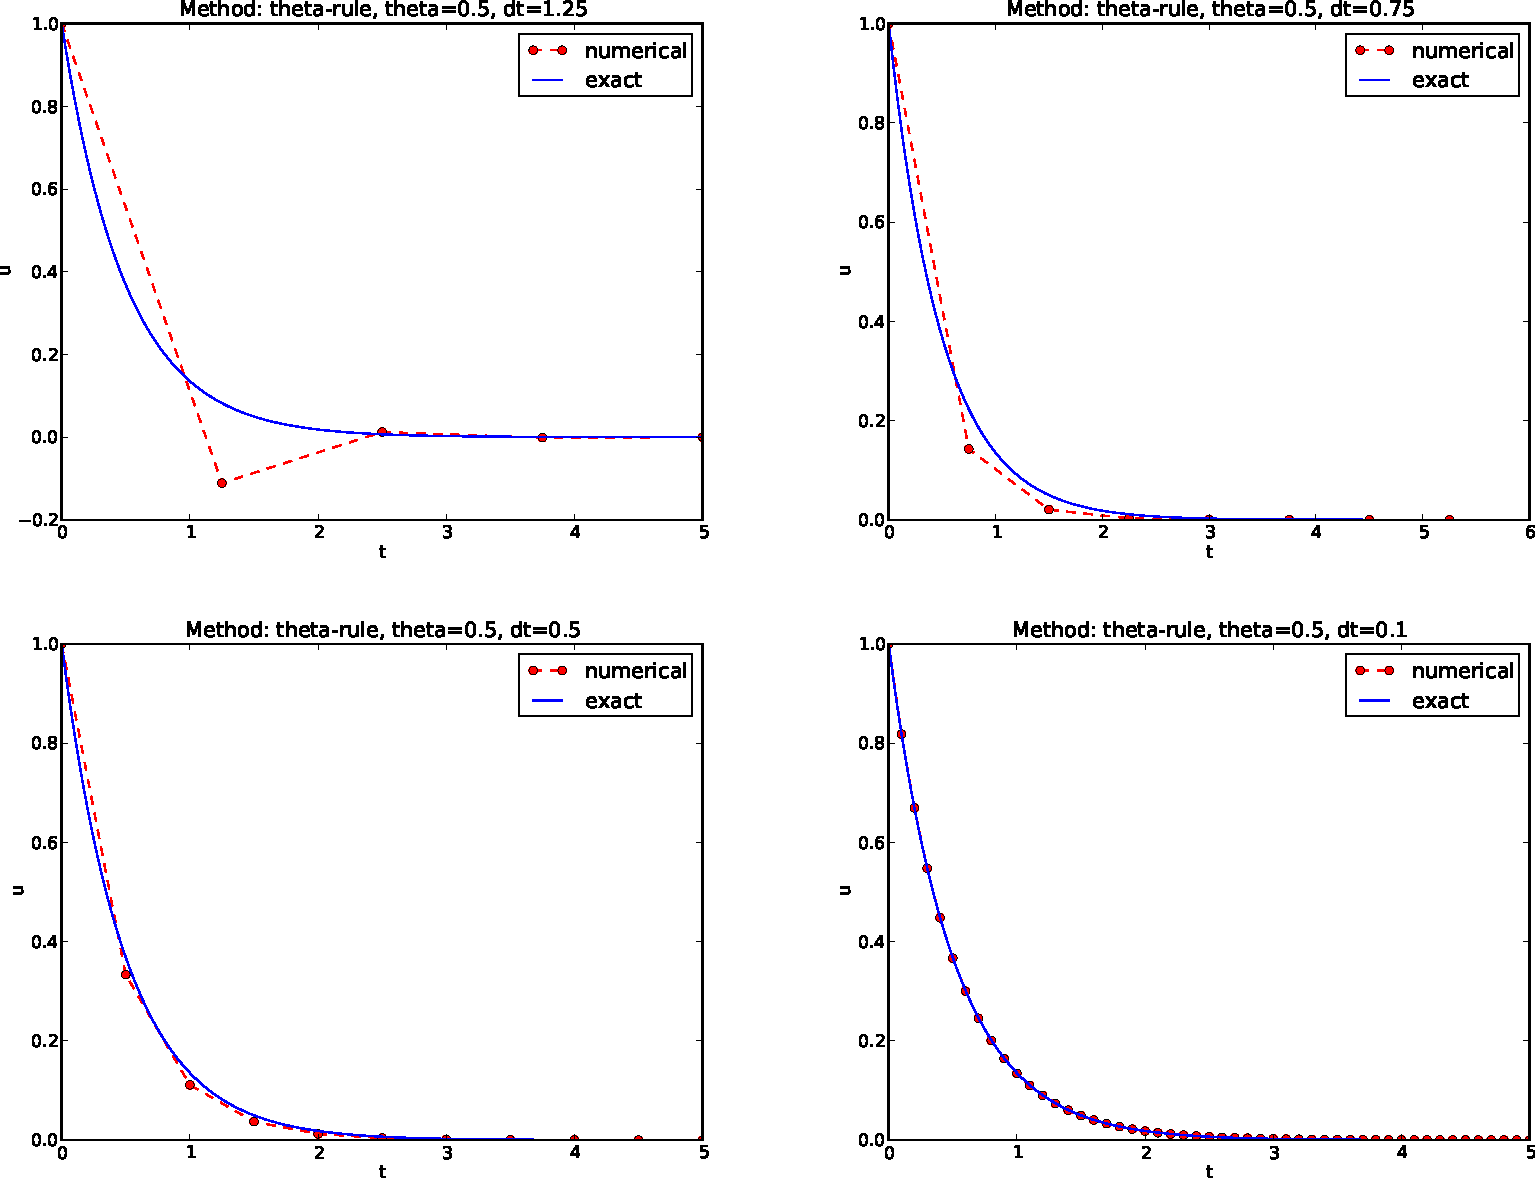
\includegraphics[width=0.9\linewidth]{../doc/src/slides/fig/CN.pdf}}
\vspace{6mm}
\end{frame}

\begin{frame}[plain,fragile]
\frametitle{The artifacts can be explained by some theory}

\pause
Exact solution of the scheme:
\[ u^n = A^n,\quad A = \frac{1 - (1-\theta) a\Delta t}{1 + \theta a\Delta t}\thinspace .\]
\begin{itemize}
\pause
 \item Stability: $|A| < 1$
\pause
 \item No oscillations: $A>0$
\pause
 \item Always for Backward Euler ($\theta=1$)
\pause
 \item $\Delta t < 1/a$ for Forward Euler ($\theta=0$)
\pause
 \item $\Delta t < 2/a$ for Crank-Nicolson ($\theta=1/2$)
\end{itemize}
\noindent
\pause
\begin{block}{Concluding remarks: }
Only the Backward Euler scheme is guaranteed to always give
qualitatively correct results.
\end{block}
\end{frame}

\end{document}
